\documentclass[12pt]{report}

\usepackage{listings} % used to insert code snippets
\usepackage{xcolor} % used to include specific colors
\usepackage{longtable}
\usepackage{textcomp}
\usepackage{subfig}
\usepackage{graphicx}

\lstset{breaklines=true}

% These are the appendices
\begin{document}

\appendix
\chapter{List of Parameters\label{app:params}}

\begin{longtable}{r l l}
\label{table:params}\\
\caption{This table gives the parameters for UO\textsubscript{2} generating the energy function.}\\
\hline
\hline
Array number & Parameter name & Parameter value \\
\hline
\endfirsthead
\multicolumn{3}{c}{\tablename\ \thetable\ -- \textit{Continued from previous page}}\\
\hline
Array number & Parameter name & Parameter value \\
\hline
\endhead
\hline
\multicolumn{3}{r}{\textit{Continued on next page.}}\\
\endfoot
\hline
\hline
\endlastfoot
1 & Energy Scaling Factor ($e_{RGB}$) & 1.6012 $J/m^2$ \\
2 & \textlangle{}100\textrangle{} Max Distance & 0.405 \\
3 & \textlangle{}110\textrangle{} Max Distance & 0.739 \\
4 & \textlangle{}111\textrangle{} Max Distance & 0.352 \\
5 & \textlangle{}100\textrangle{} Weight & 50.5 \\
6 & \textlangle{}110\textrangle{} Weight & 4.55 \\
7 & \textlangle{}111\textrangle{} Weight & 0.08 \\
8 & \textlangle{}100\textrangle{} Tilt/Twist Mix Power Law (1) & 0.03325 \\
9 & \textlangle{}100\textrangle{} Tilt/Twist Mix Power Law (2) & 0.00053125 \\
10 & Maximum \textlangle{}100\textrangle{} Twist Energy & 0.60903 \\
11 & \textlangle{}100\textrangle{} Twist Shape Factor & 1.4486 \\
12 & \textlangle{}100\textrangle{} Asymmetric Tilt Interpolation Power & 35.8 \\
13 & \textlangle{}100\textrangle{} Symmetric Tilt First Peak Energy & 1.0058 \\
14 & \textlangle{}100\textrangle{} Symmetric Tilt First $\Sigma5$ Energy & 0.84456 \\
15 & \textlangle{}100\textrangle{} Symmetric Tilt Second Peak Energy & 0.97259 \\
16 & \textlangle{}100\textrangle{} Symmetric Tilt Second $\Sigma5$ Energy & 0.9379 \\
17 & \textlangle{}100\textrangle{} Symmetric Tilt $\Sigma17$ Energy & 0.96881 \\
18 & \textlangle{}100\textrangle{} Symmetric Tilt First Peak Angle & 0.31569 \\
19 & \textlangle{}100\textrangle{} Symmetric Tilt Second Peak Angle & 0.88538 \\
20 & \textlangle{}110\textrangle{} Tilt/Twist Mix Power Law (1) & 3.1573 \\
21 & \textlangle{}110\textrangle{} Tilt/Twist Mix Power Law (2) & 1.9784 \\
22 & \textlangle{}110\textrangle{} Twist Peak Angle & 0.46145 \\
23 & \textlangle{}110\textrangle{} Twist Peak Energy & 1.1444 \\
24 & \textlangle{}110\textrangle{} Twist $\Sigma3$ Energy & 1.0931 \\
25 & \textlangle{}110\textrangle{} Twist 90\textdegree{} Energy & 1.152 \\
26 & \textlangle{}110\textrangle{} Asymmetric Tilt Shape Factor & 3.1843 \\
27 & \textlangle{}110\textrangle{} Symmetric Tilt Third Peak Energy & 1.0514 \\
28 & \textlangle{}110\textrangle{} Symmetric Tilt $\Sigma3$ Energy & 0.61703 \\
29 & \textlangle{}110\textrangle{} Symmetric Tilt Second Peak Energy & 1.0902 \\
30 & \textlangle{}110\textrangle{} Symmetric Tilt $\Sigma11$ Energy & 0.56686 \\
31 & \textlangle{}110\textrangle{} Symmetric Tilt First Peak Energy & 1.1024 \\
32 & \textlangle{}110\textrangle{} Symmetric Tilt Third Peak Angle & 0.88736 \\
33 & \textlangle{}110\textrangle{} Symmetric Tilt Second Peak Angle & 1.8711 \\
34 & \textlangle{}110\textrangle{} Symmetric Tilt First Peak Angle & 2.731 \\
35 & \textlangle{}111\textrangle{} Tilt-Twist Linear Interpolation & 38.201 \\
36 & \textlangle{}111\textrangle{} Twist Shape Factor & 1.2414 \\
37 & \textlangle{}111\textrangle{} Twist Peak Angle & 0.49979 \\
38 & \textlangle{}111\textrangle{} Twist Peak Energy & 0.7971 \\
39 & \textlangle{}111\textrangle{} Symmetric Tilt Peak Angle & 0.25966 \\
40 & \textlangle{}111\textrangle{} Symmetric Tilt Max Energy & 1.0288 \\
41 & \textlangle{}111\textrangle{} Symmetric Tilt $\Sigma3$ Energy & 1.1311 \\
42 & \textlangle{}111\textrangle{} Asymmetric Tilt Symmetry Point Energy & 3.7674 \\
43 & \textlangle{}111\textrangle{} Asymmetric Tilt Scale Factor & 0.053417 \\
\end{longtable}

\chapter{Graphs\label{app:graphs}}
\begin{figure}[ht!]
 \centering
 
 \subfloat[]{\label{appfig:compare100Twist}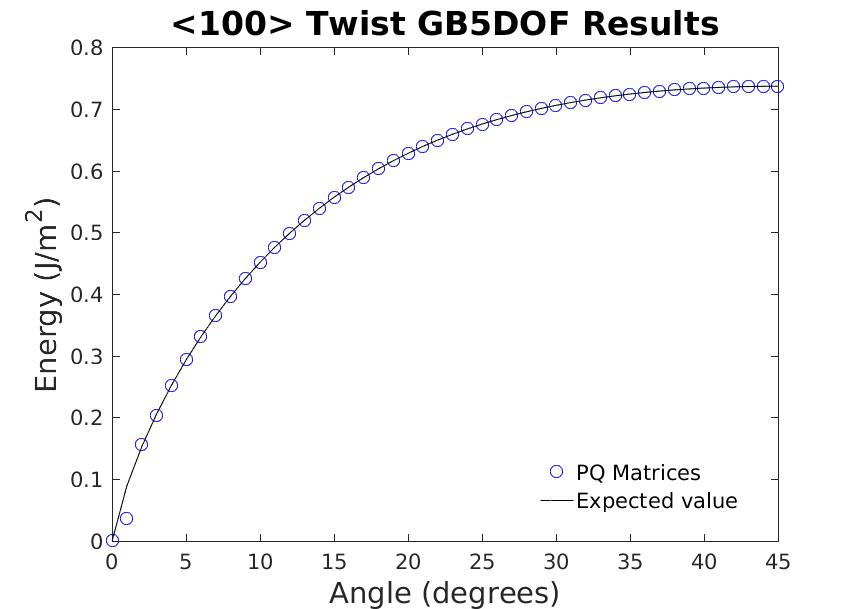
\includegraphics[scale=0.24]{Images/TestPQFit100Twist}}\quad
 \subfloat[]{\label{appfig:compare100Tilt}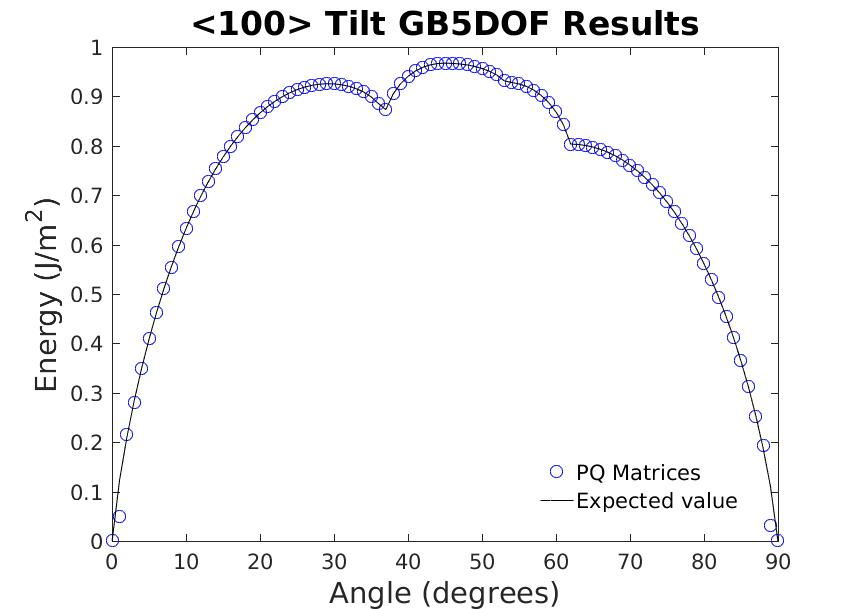
\includegraphics[scale=0.26]{Images/TestPQFit100Tilt}}
 \caption[A comparison of the \textlangle{}100\textrangle{} copper curves with the calculated results.]{\label{appfig:compare100} The \textlangle{}100\textrangle{} twist \protect\subref{appfig:compare100Twist} and tilt \protect\subref{appfig:compare100Tilt} results for the P and Q matrices as compared to Bulatov \emph{et al.}'s energy profiles. The expected value was calculated using Bulatov \emph{et al.}'s \lstinline!GB5DOF.m! MATLAB\textsuperscript{\textregistered} script with the default values.  The calculated values were found by inputting the matrices into the \lstinline!GB5DOF.m! script. With the exception of the data points at 1\textdegree{} in both \protect\subref{appfig:compare100Twist} and \protect\subref{appfig:compare100Tilt} and 89\textdegree{} in \protect\subref{appfig:compare100Tilt}, the energies calculated from the matrices matches the expected curves exactly.}
\end{figure}

\begin{figure}[ht!]
 \centering
 
 \subfloat[]{\label{appfig:compare110Twist}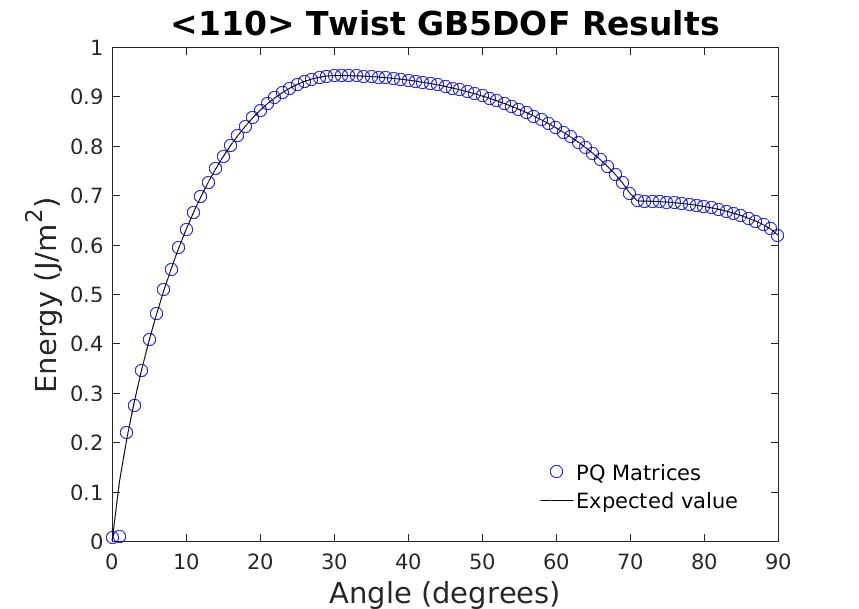
\includegraphics[scale=0.24]{Images/TestPQFit110Twist}}\quad
 \subfloat[]{\label{appfig:compare110Tilt}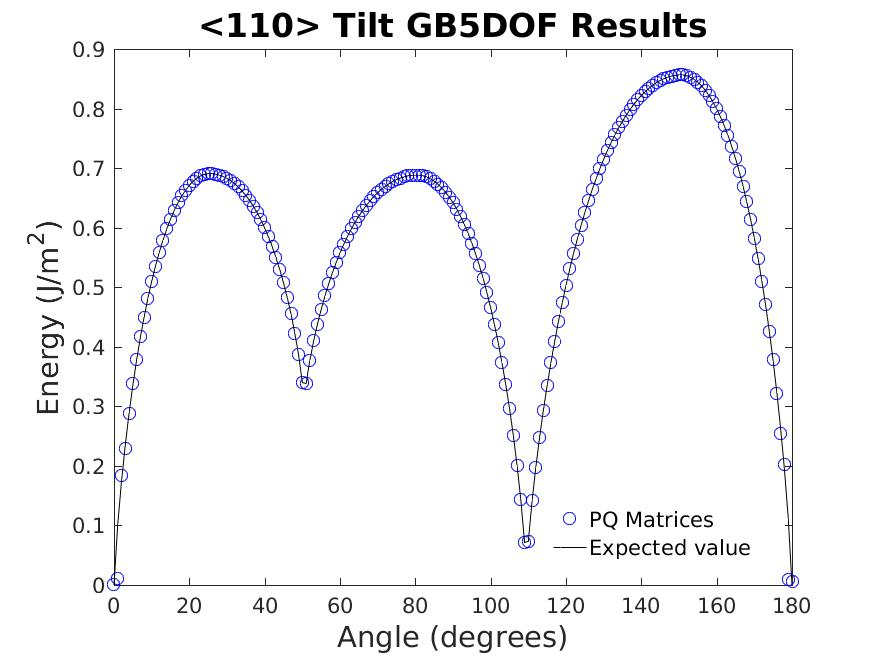
\includegraphics[scale=0.26]{Images/TestPQFit110Tilt}}
 \caption[A comparison of the \textlangle{}110\textrangle{} copper curves with the calculated results.]{\label{appfig:compare110} The \textlangle{}110\textrangle{} twist \protect\subref{appfig:compare110Twist} and tilt \protect\subref{appfig:compare110Tilt} results for the P and Q matrices as compared to Bulatov \emph{et al.}'s energy profiles. The expected value was calculated using Bulatov \emph{et al.}'s \lstinline!GB5DOF.m! MATLAB\textsuperscript{\textregistered} script with the default values.  The calculated values were found by inputting the matrices into the \lstinline!GB5DOF.m! script. With the exception of the data points at 1\textdegree{} in both \protect\subref{appfig:compare110Twist} and \protect\subref{appfig:compare110Tilt} and 179\textdegree{} in \protect\subref{appfig:compare110Tilt}, the energies calculated from the matrices matches the expected curves exactly.}
\end{figure}

\begin{figure}[ht!]
 \centering
 
 \subfloat[]{\label{appfig:compare111Twist}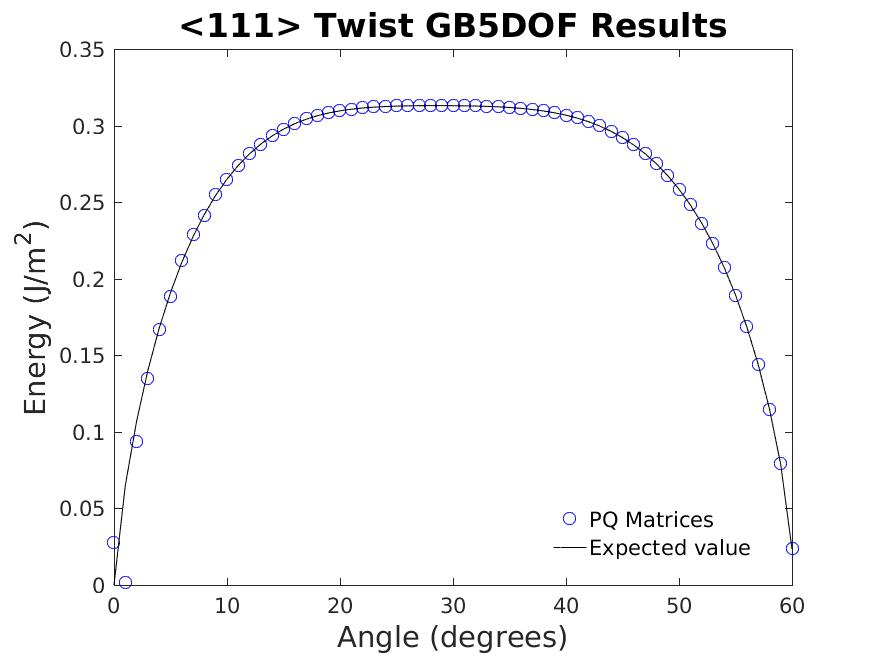
\includegraphics[scale=0.24]{Images/TestPQFit111Twist}}\quad
 \subfloat[]{\label{appfig:compare111Tilt}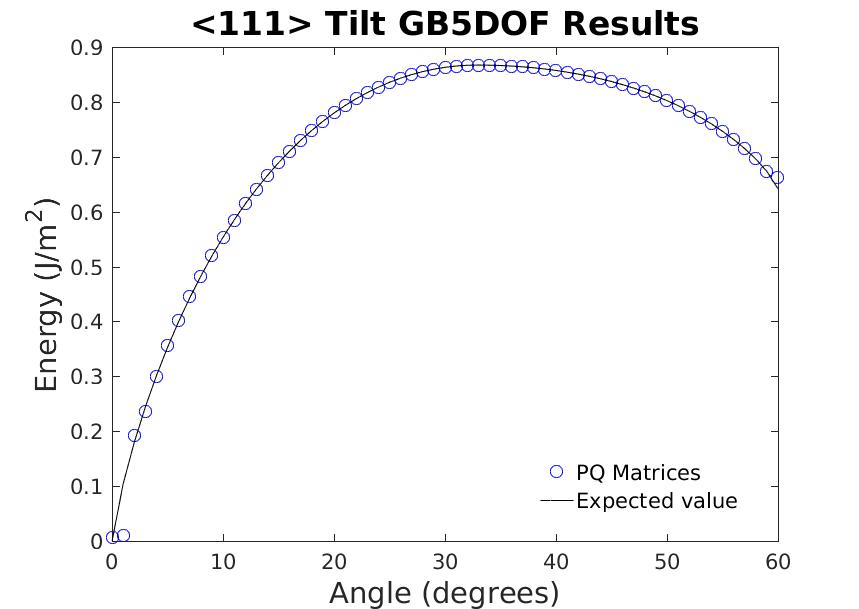
\includegraphics[scale=0.26]{Images/TestPQFit111Tilt}}
 \caption[A comparison of the \textlangle{}111\textrangle{} copper curves with the calculated results.]{\label{appfig:compare111} The \textlangle{}111\textrangle{} twist \protect\subref{appfig:compare111Twist} and tilt \protect\subref{appfig:compare111Tilt} results for the P and Q matrices as compared to Bulatov \emph{et al.}'s energy profiles. The expected value was calculated using Bulatov \emph{et al.}'s \lstinline!GB5DOF.m! MATLAB\textsuperscript{\textregistered} script with the default values.  The calculated values were found by inputting the matrices into the \lstinline!GB5DOF.m! script. With the exception of the data points at 1\textdegree{} in both \protect\subref{appfig:compare111Twist} and \protect\subref{appfig:compare111Tilt} and 60\textdegree{} in \protect\subref{appfig:compare111Tilt}, the energies calculated from the matrices matches the expected curves exactly.}
\end{figure}

\begin{figure}[ht!]
 \centering
 
 \subfloat[]{\label{appfig:100TwistPQ}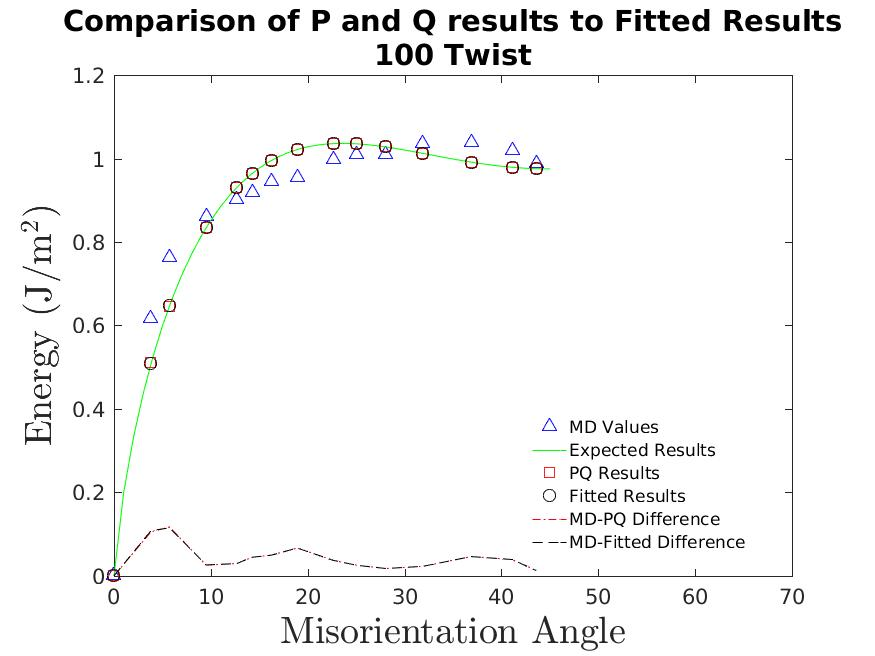
\includegraphics[scale=0.26]{Images/100TwistPQvsMD}}\quad
 \subfloat[]{\label{appfig:100TiltPQ}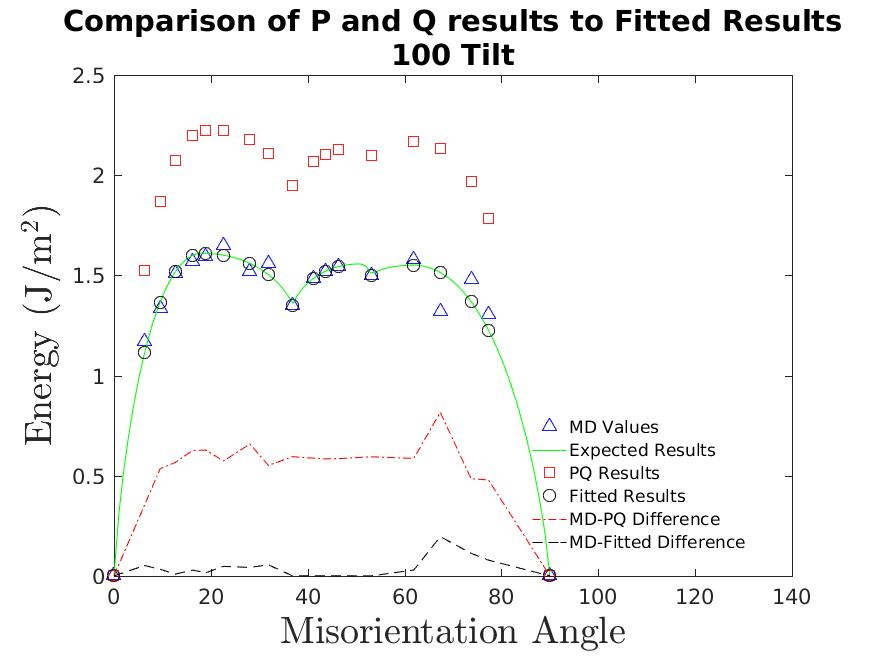
\includegraphics[scale=0.26]{Images/100TiltPQvsMD}}
 \caption[Comparison of the PQ matrices with the expected result for \textlangle{}100\textrangle{} 1D subset.]{\label{appfig:100PQ} A comparison of the expected value of the fitted function with the values calculated using the P and Q matrices for the \textlangle{}100\textrangle{} 1D subsets.  The MD values are shown for reference.  \protect\subref{appfig:100TwistPQ} PQ results follow exactly the fitted curve.  \protect\subref{appfig:100TiltPQ} has a scaling issue yet to be fixed.  It is uncertain what is causing the scaling issue for this subset.}
\end{figure}

\begin{figure}[ht!]
 \centering
 
 \subfloat[]{\label{appfig:110TwistPQ}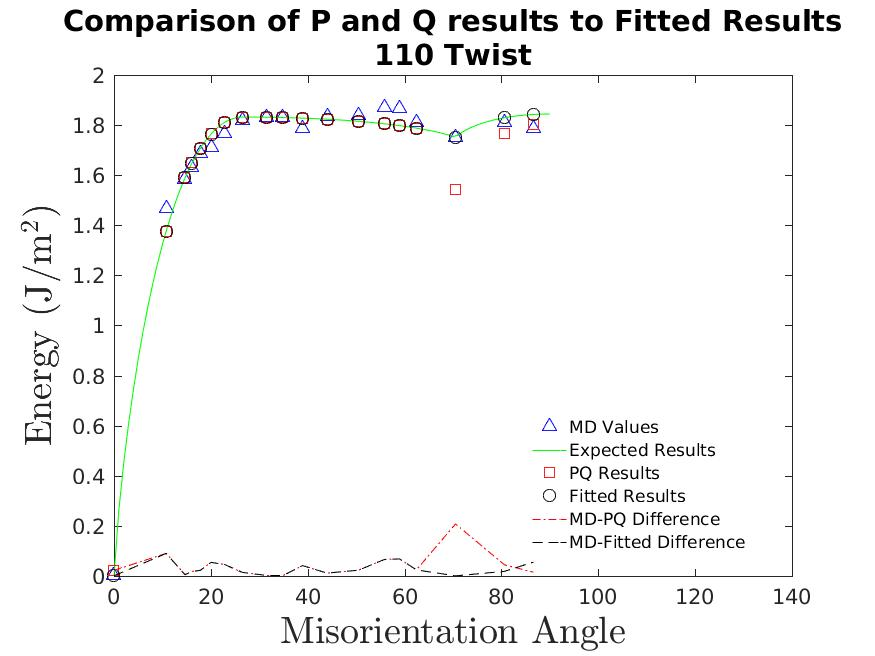
\includegraphics[scale=0.26]{Images/110TwistPQvsMD}}\quad
 \subfloat[]{\label{appfig:110TiltPQ}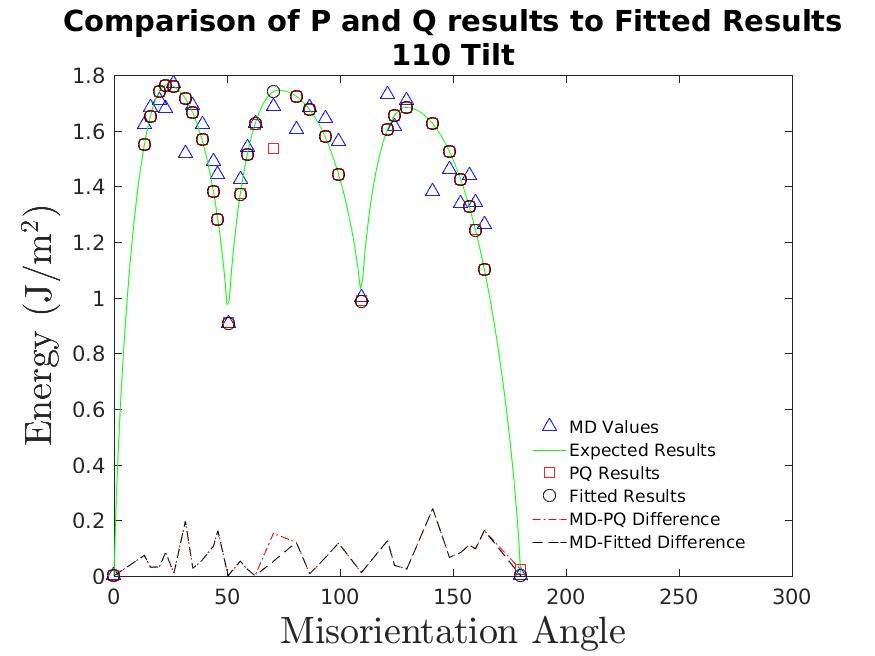
\includegraphics[scale=0.26]{Images/110TiltPQvsMD}}
 \caption[Comparison of the PQ matrices with the expected result for \textlangle{}110\textrangle{} 1D subset.]{\label{appfig:110PQ} A comparison of the expected value of the fitted function with the values calculated using the P and Q matrices for the \textlangle{}110\textrangle{} 1D subsets.  MD values are shown for reference.  \protect\subref{appfig:110TwistPQ} follows the fitted result until the cusp, at which point some anomalies appear.  The results from the PQ matrices dip well below the expected value at the cusp, and never make it back to the original fitted line. \protect\subref{appfig:110TiltPQ} has a similar issue on a lesser scale.  Only two of the calculated points do not follow the fitted curve.  The endpoint is expected to return a zero value, where the PQ matrices calculated a value slightly higher.  There is also an unexpected cusp from the PQ matrices in the middle of the second hump.  All other data points follow the fitted curve exactly.}
\end{figure}

\begin{figure}[ht!]
 \centering
 
 \subfloat[]{\label{appfig:111TwistPQ}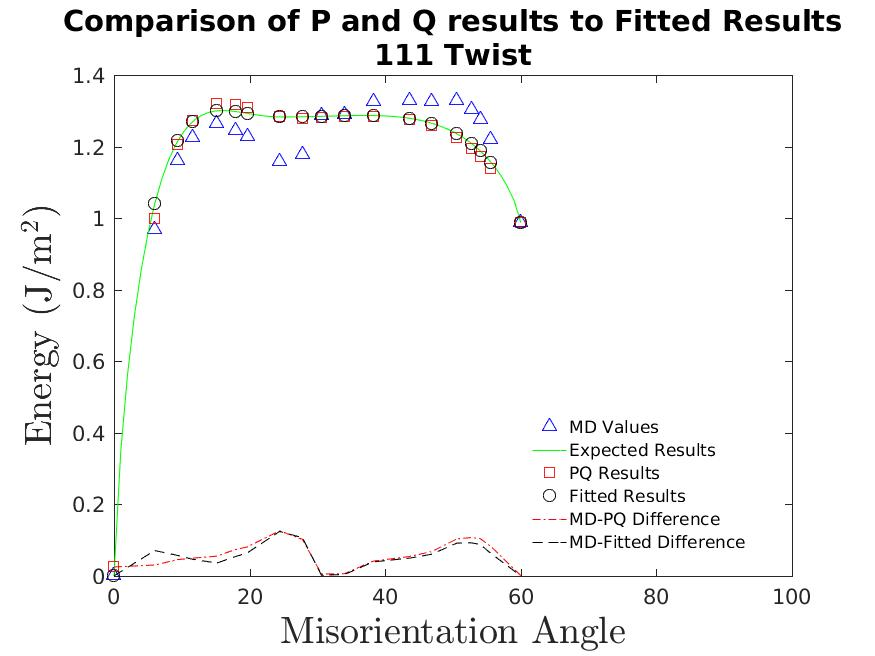
\includegraphics[scale=0.26]{Images/111TwistPQvsMD}}\quad
 \subfloat[]{\label{appfig:111TiltPQ}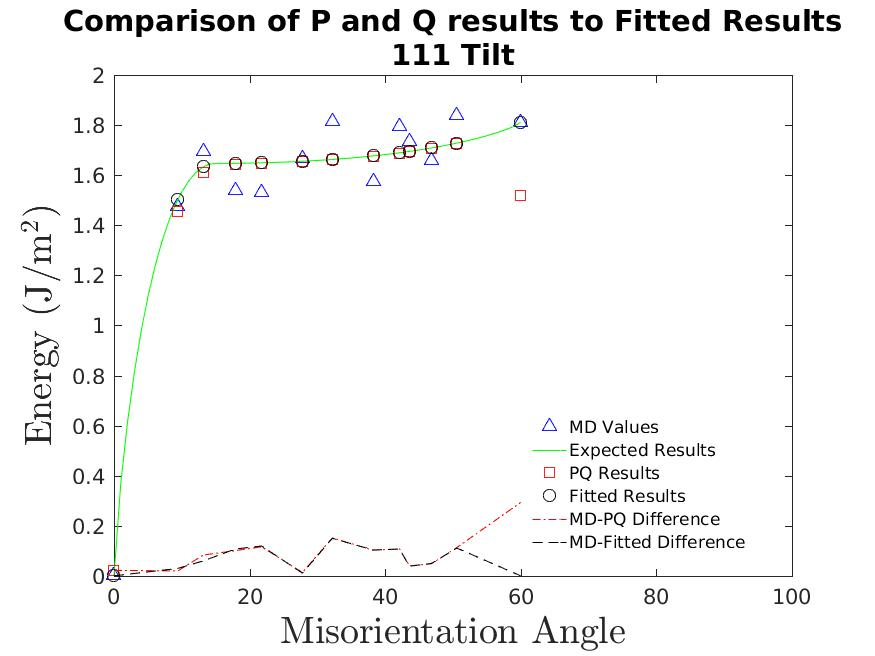
\includegraphics[scale=0.26]{Images/111TiltPQvsMD}}
 \caption[Comparison of the PQ matrices with the expected result for \textlangle{}111\textrangle{} 1D subset.]{\label{appfig:111PQ} A comparison of the expected value of the fitted function with the values calculated using the P and Q matrices for the \textlangle{}111\textrangle{} 1D subsets.  MD values are shown for reference.  \protect\subref{appfig:111TwistPQ} closely follows the expected fitted values, but has a slight error throughout.  \protect\subref{appfig:111TiltPQ} follows the expected values exactly in the center of the fitting, but misses slightly for lower angle boundaries, and misses completely at the end.}
\end{figure}

\chapter{Orientation Matrix Generator\label{app:OrientationMatrix}}
This code generates the orientation matrices (known as the P and Q matrices in Bulatov \emph{et al.}'s code). Provision for calculating the matrices one of two ways is provided in-code through the use of command-line options.

\lstinputlisting[language=Python, keywordstyle=\color{magenta}, identifierstyle=\color{blue},breaklines=true]{../../scripts/orientation_matrix.py}

\chapter{genOrientationMatrix.sh Bash Script\label{app:genOrientationMatrix}}
This bash script reads a CSV file containing misorientation angles data, and uses those angles to generate the P and Q matrices.  This script calls the script \lstinline!orientation_matrix.py!.

\lstinputlisting[language=Bash,keywordstyle=\color{magenta}, identifierstyle=\color{cyan},breaklines=true]{../../scripts/genOrientationMatrices.sh}
\end{document}